\chapter{Geração das instâncias}
  
	Atualmente existem diversas fontes na qual se podem obter instâncias para
	problemas de otimização combinatória sendo uma das mais conhecidas a
	OR-Library \footnote{ A OR-Library pode ser acessado em
	http://people.brunel.ac.uk/~mastjjb/jeb/info.html} que foi descrito
	inicialmente em J.E.Beasley \cite{orlibrary} permitindo o acesso a centenas de
	conjuntos de instâncias a partir da Internet.
  
	Apesar da existência dessas entidades não forams encontrados nenhuma instância
	que fosse compatível com o problema de construção de trilhos de aeronaves,
	fazendo-se então necessário a criação de um conjunto de instâncias próprias
	que além de permitir a conclusão desse presente trabalho ainda irá servir como
	base para futuras propostas.
  
 	Atualmente estamos trabalhando com 2 instâncias. Uma é referente à uma malha
 	diária da companhia aérea Rio-Sul, que é formada por 107 voos. Essa instância
 	foi obtida a partir de um relatório técnico da Universidade Federal do Rio de
 	Janeiro \cite{pontes2002} e adaptada para corresponder as características
 	necessárias do nosso modelo.
 	 	
	A outra instância trabalhada é a da empresa de transporte aéreo brasileira
	denomidada TAM (http://www.tam.com.br). A obtenção desses  dados foi feita
	através da seleção manual do conjunto de voos que ela operava em dezembro de
	2010. Foram selecionados os voos operados pelo equipamento AirBus Industrie
	A310 que tinham o horário de partida iniciando em uma segunda-feira que foi
	identificada como sendo o dia 0 (zero) apenas para permitir sua utilização no
	algoritmo. Essa instância que foi obtida é composta por 241 voos e possui uma
	grande quantidade de ligações entre os 31 aeroportos envolvidos tornando o
	grau de complexidade mais elevado que instâncias com a características 
	hub-and-spoke que é mais comum nas malhas comerciais norte-americanas.
	
	Uma malha é considerada como sendo \textit{hub-and-spoke} quando existe uma
	grande concentração de voos em poucos aeroportos como pode ser visto na Figura
	\ref{fig:hubandspoke}.
	
\begin{figure}[ht]
\caption{Malha hub-and-spoke. \mbox{Fonte: (Própria)}}
\label{fig:hubandspoke}
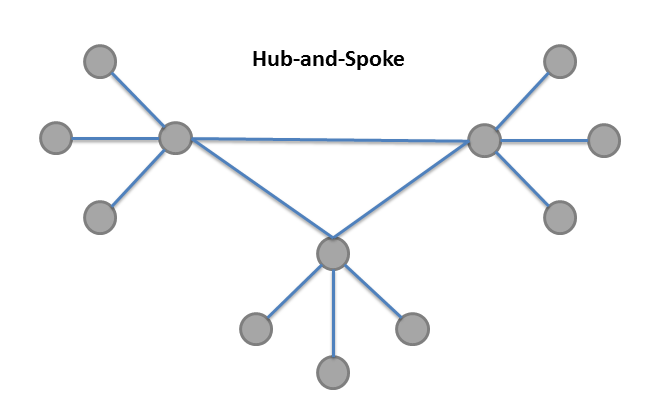
\includegraphics[scale=0.35]{./img/hubandspoke}
\end{figure}
  
%	Para se obter um limite inferior dessas instâncias foi feita uma verificação com o algoritmo do Anexo X que permite checar a %quantidade mínima de voos que colidem em uma determinada janela de tempo que é definida pelo atraso máximo permitido. (Pode-se fazer uma %formula para explicar esse funcionamento). Essa quantidade é dito como sendo o limite inferior da instância e é garantido que não existe %solução com uma melhor quantidade de trilhos que essa sem que nenhum vôo seja excluído.
  
%	A TAM tinha disponível nessa época com N aeronaves desse tipo, logo acreditamos que esse é o número de aeronaves que era necessário %para atender a todos esses voos, fazendo com que reduzir essa quantidade de voos se tornasse um dos objetivos desse trabalho.
  
	Diversas instâncias também serão geradas a partir dessa, variando o número de voos e as características das malhas com a finalidade de gerar instâncias com um variado grau de complexidade. Algum esforço também está sendo voltado para a obtenção de novas instâncias reais, porém pela falta de colaboração das empresas de transporte aéreo esse trabalho se torna demorado.
	
	%Essas instâncias podem ser vistas no Anexo N e podem ser solicitadas diretamente com o autor, porém existe a intenção de adicionar esse conjunto de instâncias na OR-Library.
  
  